\documentclass[conference]{IEEEtran}
\IEEEoverridecommandlockouts
\usepackage{biblatex}
\addbibresource{biblatex.bib}
\usepackage{amsmath,amssymb,amsfonts}
\usepackage{algorithmic}
\usepackage[utf8]{inputenc}
\usepackage[spanish, es-tabla]{babel}
\usepackage[hidelinks]{hyperref}
\usepackage{graphicx}
\usepackage{textcomp} 
\usepackage{xcolor}
\usepackage{tabularx,booktabs}
\usepackage{float}
\usepackage{graphicx}
\graphicspath{ {./} }

\newcolumntype{C}{|>{\centering\arraybackslash}X} % centered version of "X" type
\setlength{\extrarowheight}{1pt}

\begin{document}

\title{Ishvel: un Framework para la Elaboración de Tareas en Cursos Introductorios de Programación \\
}

\author{\IEEEauthorblockN{Gonzalo Fernández C.}
\IEEEauthorblockA{\textit{Departamento de Informática} \\
\textit{Universidad Técnica Federico Santa María}\\
Santiago, Chile \\
gonzalo.fernandezc@sansano.usm.cl}}

\maketitle

\begin{abstract}
Las tareas son parte importante de un curso introductorio de programación, ya que miden el aprendizaje del estudiante, mientras pone en práctica el conocimiento adquirido. Un curso introductorio requiere elaborar varias tareas por semestre, y se debe velar porque estas sean de calidad, ya que impactan enormemente en el interés del estudiante por aprender a programar. Es por esto que se propone Ishvel, un framework que, de manera metodológica, le facilite a los profesores el proceso de elaboración de tareas en cursos introductorios de programación, mientras garantiza la calidad de las mismas.
\end{abstract}

\begin{IEEEkeywords}
elaborar tareas, framework, curso introductorio de programación, educación
\end{IEEEkeywords}

\section{Objetivos}

\subsection*{Objetivo General}

\begin{itemize}
    \item Desarrollar un Framework \footnote{Marco de trabajo que plantea una metodología validada y un conjunto de herramientas, las cuales están diseñadas para la correcta aplicación de dicha metodología} para la elaboración de tareas en cursos introductorios de programación
\end{itemize}

\subsection*{Objetivos Específicos}

\begin{itemize}
    \item Identificar y definir criterios que puedan ser usados para evaluar una tarea.
    \item Definir una métrica que permita evaluar una tarea de acuerdo al cumplimiento de criterios.
    \item Definir una metodología para la elaboración de tareas utilizando el framework Ishvel.
    \item Validar cómo la aplicación de la metodología definida elabora mejores tareas.
\end{itemize}

\section{Definición Inicial del Problema}

Los cursos introductorios de programación son, en general, el primer acercamiento de un estudiante al mundo de la programación, y por lo tanto, se debe velar porque se desarrollen de la manera más prolija posible, considerando entre otras cosas, la elaboración y uso de tareas de calidad. Las tareas son parte importante del proceso de aprendizaje y enseñanza \cite{texasU}, pues permiten medir el aprendizaje de los estudiantes y proporcionarles una retroalimentación significativa \cite{NAP12636}. Además, en los cursos introductorios de programación, son la principal actividad en donde los estudiantes ponen en práctica lo que han aprendido sobre programación, lo que hace que las tareas jueguen un rol importante en su interés por aprender, pudiendo llevar al estudiante tanto a querer sobresalir resolviendo las evaluaciones del curso, como a desertar debido a su percepción de la programación por tareas de mala calidad \cite{10.5555/1968521.1968545, 10.1145/2526968.2526982}, entre otros efectos como los mencionados en el Árbol del Problema (ver Figura \ref{arbolito}).

\begin{figure}[H]
    \centering
    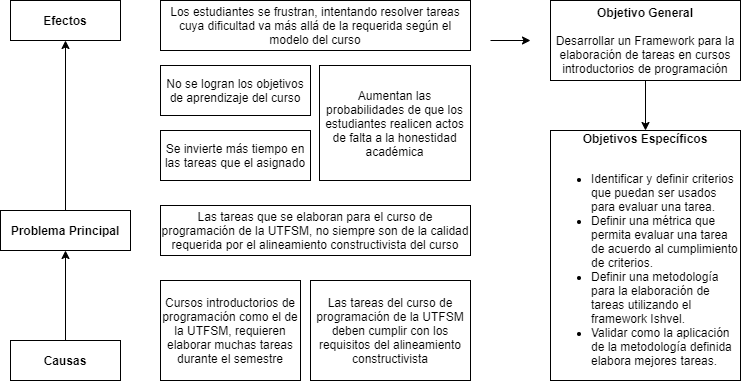
\includegraphics[width=0.49\textwidth]{arbolito.png}
    \caption{Árbol del Problema. Fuente: Elaboración propia.}
    \label{arbolito}
\end{figure}

En la Universidad Técnica Federico Santa María (UTFSM), se dicta un curso introductorio de programación a lo largo de todos sus campus. Este recibe de forma masiva a todos los estudiantes de primer año de ingeniería, y se dicta de igual forma independiente del campus o carrera del estudiante. El curso, que se lleva a cabo de forma online, está dividido en Unidades Virtuales de Aprendizaje (UVA), las cuales estructuran las actividades de cada semana (ver Figura \ref{modeloiwi}), y su diseño se basa en el alineamiento constructivista \cite{book}. Este último plantea la necesidad de que las evaluaciones del curso reflejen los objetivos de aprendizaje del mismo y, que a su vez, sean estos los que definan las actividades y tareas a realizar. Esto brinda a las tareas un rol tanto formativo como sumativo de evaluar, y requiere que estas cumplan ciertos estándares para justificar que cumplen con los objetivos de aprendizaje \cite{book}. 

\begin{figure}[H]
    \centering
    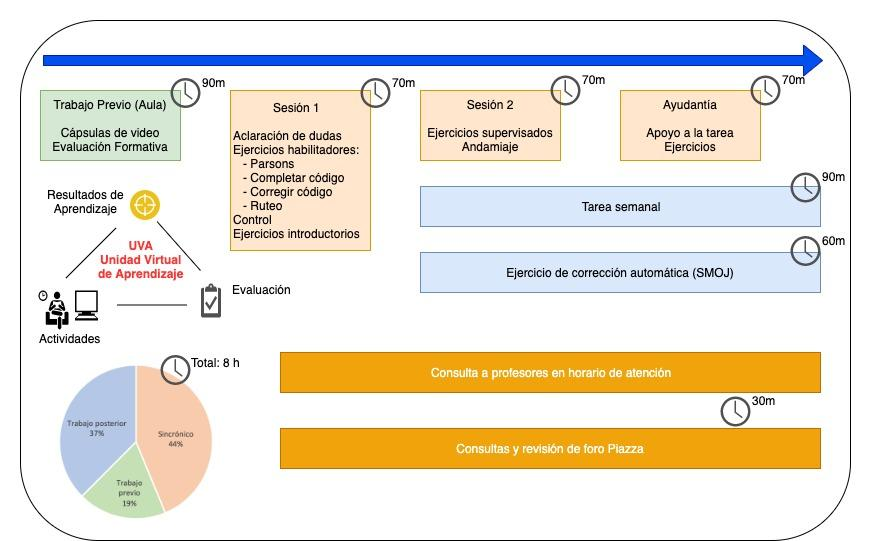
\includegraphics[width=0.47\textwidth]{uva.png}
    \caption{Modelo Formativo IWI-131. Fuente: Reglas del curso de programación de la UTFSM (2021-2).}
    \label{modeloiwi}
\end{figure}

Sin embargo, pese a que el curso cuenta con una gran cantidad de profesores, no son más de 5 los que se encargan de proponer tareas a la coordinación. Y, dado que cada semana se requiere una nueva tarea para la UVA en curso, se vuelve complicado elaborar tareas de calidad a tiempo, que cumplan con el alineamiento constructivista del curso, y que cuya resolución no requiera más tiempo que el estipulado en la UVA. Además, la elaboración de tareas se lleva a cabo sin métricas que permitan medir la calidad de cada una, o una metodología de elaboración de tareas que garantice la calidad de las mismas en el tiempo.

Entre los problemas que puede conllevar el uso de tareas que no son de calidad, se encuentran:

\begin{itemize}
    \item Pérdida del interés en aprender a programar \cite{10.1145/1227504.1227466}, de modo tal que el estudiante deje de ver el ramo como un curso de aprendizaje, y su actitud hacia él sea nétamente para aprobar.
    \item Frustración a lo largo del ramo, al punto en que el estudiante puede decidir desertar del curso y de la programación en general \cite{10.1145/2526968.2526982}.
    \item Aumentar las probabilidades de que los estudiantes realicen actos que falten a la honestidad académica para resolverla \cite{10.1145/3013499.3013507}.
    \item Complicar la elaboración de la rúbrica con la cual la tarea será evaluada, lo que puede conllevar a entregar un feedback menos valioso al estudiante 
\end{itemize}

Es por esto que se requiere de un marco de trabajo que permita elaborar tareas de calidad, el cual brinde tanto una metodología como herramientas que faciliten a los profesores esta labor, ahorrándoles tiempo y garantizando a los estudiantes del curso una mejor experiencia de aprendizaje.

\section{Discusión Bibliográfica Preliminar}

Diversos autores han abordado la elaboración y medición de tareas de calidad, enfocándose tanto en factores emocionales del estudiante \cite{10.1145/1839594.1839609, 10.1145/1227504.1227466, 10.5555/1968521.1968545, 10.1145/2526968.2526982}, como en aspectos particulares de cualquier tarea en sí \cite{texasU, 10.1145/2676723.2677276, 10.1145/1140124.1140167}. Y en general, siempre se destacan 3 aspectos principales:

\begin{itemize}
    \item Las tareas deben tener alguna aplicación real, o bien, resolver un problema real que le dé sentido al tiempo que el estudiante invertirá en resolverla.
    \item Las tareas deben ser interesantes, un problema puede expresarse utilizando un contexto de la actualidad, de lo que los estudiantes en general considerarían interesante como lo son sus bandas, juegos, tendencias, etc.
    \item Las tareas deben tener un nivel de dificultad adecuado, ni muy difíciles como para frustrar al estudiante, ni muy fáciles como para no cumplir con los objetivos de aprendizaje de la misma.
\end{itemize}

Por lo tanto, lo que se busca con el framework a desarrollar, es establecer un marco de trabajo que garantice elaborar una tarea que cumpla con, al menos, aquellos 3 aspectos. Un primer enfoque sería que el framework elaborara automáticamente la tarea, sin embargo, proyectos como Moulinog \cite{10.1145/3414080.3414100} han sido muy limitados en lograr esto, pues están limitados a, en base a 1 tarea, generar múltiples tareas que son en esencia lo mismo con la salvedad de cambiar ciertos valores y palabras, que no garantizan que 1 misma solución no sea esencialmente capaz de resolver 2 tareas distintas de las generadas.

Sin embargo, la idea de tener tareas base motiva a investigar acerca de si es buena idea re-utilizar tareas, generando un pequeño banco de tareas de calidad, pero teniendo en cuenta que éstas deben ser del tipo \textit{Tweakable assignments} \cite{10.1145/3477429}, es decir, la mayoría de sus partes pueden re-utilizarse, a excepción de ciertas partes las cuales, en base a ciertas especificaciones, deben modificarse en la nueva tarea de modo tal que una solución a la tarea original, simplemente no funcione con la tarea nueva que se está elaborando, manteniendo así la calidad de la tarea original, y evitando llegar a aumentar las probabilidades de actos fraudulentos por parte de los estudiantes, quienes pueden hacerse de las soluciones de tareas anteriores \cite{10.1145/3013499.3013507}.

Dicho esto, la forma en que el framework debiese funcionar, es primero presentando al profesor la metodología con la cual elaborar la tarea, y segundo, brindarle una herramienta que le permita al profesor, tanto observar métricas de utilidad a medida que redacta, como una validación de que los objetivos de aprendizaje esperados para esa tarea, se cumplan en base a diversas validaciones, como lo sería la revisión del código que resuelve el problema, entre otros. 

El framework además de definir métricas que pueda medir de forma automátizada sobre cualquier tarea, también debe ofrecer de forma sencilla una manera de que la tarea, una vez haya sido aplicada, sea evaluada por otros actores. Existen diversos componentes que pueden apoyar en esta evaluación posterior, cada uno con diversos porcentajes de desempeño en base a la cantidad de datos de medición que pueden aportar \cite{NAP12636}. Ésta obtención de retroalimentación sobre la tarea se puede obtener mediante formularios auto-generados por el framework, así como su posterior análisis debe ser condensado de manera automática para así estar al tanto de las fortalezas y debilidades de la tarea, según la percepción de estudiantes y profesores, principalmente en la resolución de la misma por parte del estudiante, como en su elaboración por parte del profesor.

\section{Plan de Trabajo}

\begin{table}[!h]
    \centering
    \scalebox{0.85}{\begin{tabular}{|l|c|}
        \hline 
        \textbf{Actividad} & \textbf{Semanas}\\
        \hline
        Elaboración del Estado del Arte & 2\\
        \hline
        Recopilar criterios que permitan evaluar la calidad de una tarea & 1\\
        \hline
        Definir métricas que permitan evaluar la calidad de una tarea & 1\\
        \hline
        Definir los casos de uso del framework Ishvel & 1\\
        \hline
        Analizar todas las tareas disponibles del curso de programación UTFSM & 1\\
        \hline
        Elaborar y probar prototipos del framework & 1\\
        \hline
        Documentar la metodología del framework Ishvel & 1\\
        \hline
        Implementación del framework para elaborar las tareas de programación & 8\\
        \hline
        Análisis de resultados & 2\\
        \hline
        Elaboración del documento de memoria & 3\\
        \hline
        Correcciones finales & 1\\
        \hline
        \textbf{Total} & \textbf{22}\\
        \hline
    \end{tabular}}
    \caption{Actividades del Plan de Trabajo. Fuente: Elaboración propia}
    \label{tab:plan} 
\end{table}

\section{Tiempos SCT}

\begin{table}[H]
    \centering
    \begin{tabular}{|l|c|}
        \hline 
        \textbf{Actividad} & \textbf{Tiempo [hrs]}\\
        \hline
        Planificación & 2\\
        \hline
        Búsqueda de información & 3\\
        \hline
        Análisis & 15\\
        \hline
        Desarrollo & 10\\
        \hline
        Edición & 1\\
        \hline
        Desarrollo del video & 3\\
        \hline
        \textbf{Total} & \textbf{39}\\
        \hline
    \end{tabular}
    \label{tab:actividades} 
    \caption{Tabla de Tiempos SCT.}
\end{table}

\section{Video}

Youtube: \url{https://youtu.be/4SkeVD_pvVw}

\printbibliography
\end{document}